%Optics Homework_4
\documentclass[10pt,a4paper]{article}
\usepackage[UTF8]{ctex}
\usepackage{bm}
\usepackage{amsmath}
\usepackage{extarrows}
\usepackage{amsthm}
\usepackage{amssymb}
\usepackage{graphicx}
\usepackage{multirow}
\title{光学作业\#4}
\author{陈稼霖 \and 45875852}
\date{2018.11.04}
\begin{document}
\maketitle
\section*{3-1}解:
$F$蓝线的干涉条纹间距为
\[
\Delta x_F = \frac{\lambda_FD}{d} = \frac{486.1\times10^{-9}m\times3m}{0.1\times10^{-3}m} = 1.46\times10^{-2}m = 14.6mm
\]
$D$黄线的干涉条纹间距为
\[
\Delta x_D = \frac{\lambda_DD}{d} = \frac{589.3\times10^{-9}m\times3m}{0.1\times10^{-3}m} = 1.77\times10^{-2}m = 17.7mm
\]
$C$红线的干涉条纹间距为
\[
\Delta x_C = \frac{\lambda_CD}{d} = \frac{656.3\times10^{-9}m\times3m}{0.1\times10^{-3}m} = 1.97\times10^{-2}m = 19.7mm
\]
\section*{3-4}解:
当$B$逐渐拉开到$d = 16.0cm$时,管口$O$处的声音第一次消失,说明此时$B$ 股声波多走的声程($2d$)即为声波的半个波长
\[
2d = \frac{\lambda}{2}
\]
解得此声波的波长为
\[
\lambda  = 64.0cm
\]
\section*{3-5}
\subsection*{(1)}解:
干涉条纹的间距为
\begin{align*}
\Delta x &= \frac{\lambda(B + C)}{2\alpha B} = \frac{600.0\times10^{-9}m\times(0.1m + 2.1m)}{2\times\frac{\pi}{540}\times0.1m}\\
&= 1.13\times10^{-3}m = 1.13mm
\end{align*}
\subsection*{(2)}解:
幕上两束光的交叠区宽度为
\[
\Delta l = 2\alpha C = 2\times\frac{\pi}{540}\times2.1m = 2.44\times10^{-2} = 24.4mm
\]
$\frac{\Delta l}{\Delta x} \approx 22$,故在幕上最多能看到$22$条干涉条纹。
\subsection*{(3)}解:
如果光源到两镜交线的距离增大一倍,干涉条纹的间距变为
\begin{align*}
\Delta x &= \frac{\lambda(B' + C)}{2\alpha B'} = \frac{600.0\times10^{-9}m\times(0.2m + 2.1m)}{2\times\frac{\pi}{540}\times0.2m}\\
&= 5.9\times10^{-4}m = 0.59mm
\end{align*}
大约为原来的$\frac{1}{2}$。
\subsection*{(4)}答:
如果光源与两镜交线的距离保持不变,而在横向有所移动,干涉条纹的间距不变,但位置发生平移。例如光源横向移动$\delta s$,则光源关于两镜的虚像也一起平移$\delta s$,且与双镜交线的距离保持不变,干涉条纹平移$\frac{C\delta s}{B}$。
\subsection*{(5)}解:
如果要在幕上出现有一定衬比度的干涉条纹,允许缝光源的最大宽度为
\[
b = \frac{B}{2\alpha B}\lambda = \frac{1}{2\alpha}\lambda = \frac{1}{2\times\frac{\pi}{540}}\times600.0\times10^{-9}m = 5.2\times10^{-5}m = 0.052mm
\]
\section*{3-6}解:
从焦点处光源发出的光经薄透镜后变为平行光束,经过双棱镜的底,不发生偏转,经过棱镜的腰,折射,入射角为$\alpha = 3'30''$,根据斯涅耳定律
\[
n\sin\alpha = \sin(\alpha + \theta)
\]
做小角近似,解得出射光线偏转角度为
\[
\theta = (n - 1)\alpha
\]
幕上条纹的间距为
\[
\Delta x = \frac{1}{2\theta}\lambda = 4.9\times10^{-4}m = 0.49mm
\]
幕上两束光的交叠区域宽度为
\[
\Delta l = 2\theta D = 5.1\times10^{-3}m = 5.1mm
\]
$\frac{\Delta l}{\Delta x} \approx 10$,故幕上能出现$10$根干涉条纹。
\section*{3-8}
\subsection*{(1)}解:
如图(\ref{3-8}),过点$S$做经过$L_1$最上端的光线,交光轴于点$S_1'$,过点$S$做经过$L_2$最下端的光线,交光轴于点$S_2'$,两束光线交于点$S$,小三角形$\vartriangle$即为相干光束的交叠区域。
\begin{figure}[h]
\centering
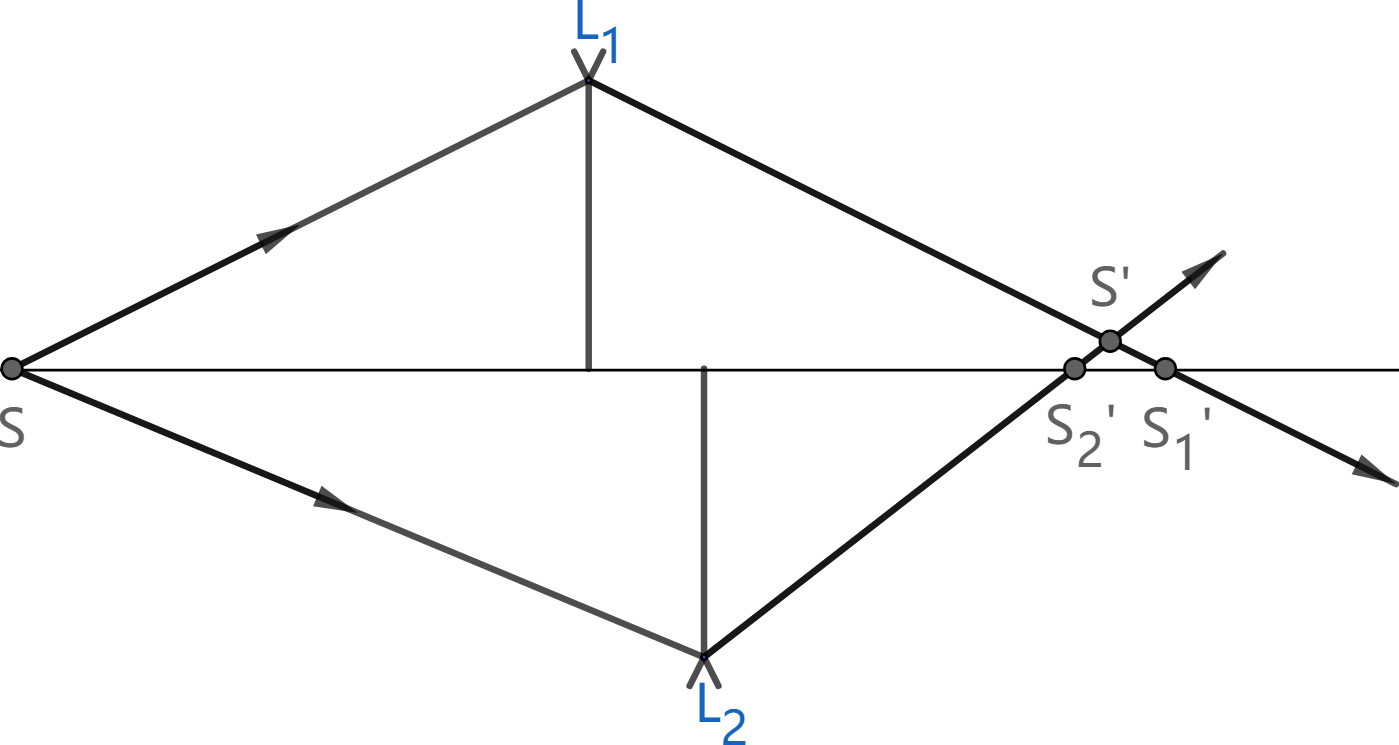
\includegraphics[scale=.2]{Homework_4_3-8(tailored).png}\\
\caption{题3-8图}\label{3-8}
\end{figure}
\subsection*{(2)}答:
幕上的条纹应为一系列同心的半圆环。
\subsection*{(3)}
根据薄透镜成像公式,$S$发出的光线经$L_1$成像于$S_1'$
\[
\frac{1}{s_1'} + \frac{1}{s_1} = \frac{1}{f}
\]
代入$f = 30cm, s_1 = 60cm$,解得$S_1'$与$L_1$之间的距离为
\[
s_1' = 60cm
\]
$S$发出的光线经$L_2$成像于$S_2'$
\[
\frac{1}{s_2'} + \frac{1}{s_2} = \frac{1}{f}
\]
代入$f = 30cm, s_2 = 60cm + 2cm = 62cm$,解得$S_2'$与$L_2$之间的距离为
\[
s_2' = 58.125cm
\]
故两像间的中点与$L_2$的距离为$(60 - 2 + 58.1) / 2 = 58.063cm$。

若在此放一光轴,可以视为$S_1'$和$S_2'$两个相干点光源在过其中点且与光轴垂直的平面上干涉成像,$S_1'$和$S_2'$与中点之间的距离为$d = [58.125 - (60 - 2)] / 2 = 0.063cm = 0.63mm$,故在屏幕上第$n$级圆环与第$(n + 1)$ 级圆环之间的半径差为
\begin{align*}
\Delta x_n &= \sqrt{[d + (n + 1)\frac{\lambda}{2}]^2 - d^2} - \sqrt{(d + n\frac{\lambda}{2})^2 - d^2}\\
&= \sqrt{2(n + 1)d\frac{\lambda}{2} + (n + 1)^2(\frac{\lambda}{2})^2} - \sqrt{2nd\frac{\lambda}{2} + n^2(\frac{\lambda}{2})^2}
\end{align*}
由于$\lambda\ll d$,故可略去$\lambda^2$项近似为
\[
\Delta x_n = \sqrt{(n + 1)d\lambda} - \sqrt{nd\lambda} = \sqrt{d\lambda}(\sqrt{n + 1} - \sqrt{n}) = 0.018(\sqrt{n + 1} - \sqrt{n})mm
\]
\section*{3-9}
\subsection*{(1)}答:
干涉条纹向上移动。
\subsection*{(2)}解:
因条纹上移增加的光程和因容器处中折射率增大而增加的光程(即$20$个光的波长)相同
\[
(n - 1.000276)l = 20\lambda
\]
解得待测气体的折射率
\[
n = 1.000865
\]
\section*{3-14}
\subsection*{(1)}解:
等厚干涉,两条干涉条纹之间的高度差等于一个波长
\[
\Delta x = \frac{\lambda}{2\alpha} = \frac{\lambda}{2\frac{\Delta h}{d}}
\]
代入$\Delta x = 5\times10^{-4}m, \lambda = 589.3\times10^{-9}m, d = 5\times10^{-2}m$,解得块规$G_2$和$G_1$的高度之差为
\[
\Delta h = 2.947\times10^{-5}m = 29.47\mu m
\]
判断谁长谁短:用力按压透明平板$T$中部,若
\begin{itemize}
  \item 块规$G_2$高于$G_1$,则$T$与$G_1$之间的夹角减小,高度变化二分之一个波长对应的距离增大,$G_1$处条纹间距变宽
  \item 块规$G_2$低于$G_1$,则$T$与$G_1$之间的夹角减小,高度变化二分之一个波长对应的距离减小,$G_1$处条纹间距变密
\end{itemize}
\subsection*{(2)}解:
\begin{align*}
\Delta x &= \frac{\lambda}{2\alpha}\\
\Longrightarrow \alpha &= 2.12''\\
\Delta x' &= \frac{\lambda}{2\alpha'}\\
\Longrightarrow \alpha' &= 3.54''
\end{align*}
这说明可能存在以下四种情况
\begin{itemize}
  \item 块规$G_2$右侧高于$G_1$$29.47\mu m$,且块规$G_2$自身右侧高于左侧,倾角为$3.54'' - 2.12'' = 1.42''$
  \item 块规$G_2$右侧高于$G_1$$29.47\mu m$,且块规$G_2$自身右侧低于左侧,倾角为$3.54'' + 2.12'' = 5.66''$
  \item 块规$G_2$右侧低于$G_1$$29.47\mu m$,且块规$G_2$自身右侧低于左侧,倾角为$3.54'' - 2.12'' = 1.42''$
  \item 块规$G_2$右侧低于$G_1$$29.47\mu m$,且块规$G_2$自身右侧高于左侧,倾角为$3.54'' + 2.12'' = 5.66''$
\end{itemize}
\section*{3-16}解:
该种测量方法的原理是等厚干涉。

对于$a$,硅片之间和半反射膜之间形成尖劈形空气薄膜,单色光从正上方垂直入射,分别经过空气薄膜上下表面反射的光线重新交叠后,由于两者光程相差两倍的空气薄膜厚度,发生干涉。由于空气薄膜的厚度沿着硅片斜面向下方向均匀增大,故形成平行于硅片斜面的、等间距的干涉条纹。

对于$b$,硅片之间和半反射膜之间形成空气薄膜,单色光从正上方垂直入射,分别经过空气薄膜上下表面反射的光线重新交叠后,由于两者光程相差两倍的空气薄膜厚度,发生干涉。在左侧由于空气薄膜的厚度沿着硅片斜面边缘线均匀增大,故形成垂直于硅片斜面边缘线的等间距的干涉条纹;在右侧,由于空气薄膜的厚度沿着硅片斜面向斜下方向均匀增大,故形成斜向的、等间距的干涉条纹。
\subsection*{(2)}解:
图$b$中,$A,B$之间恰好夹有一条完整的斜条纹,故$A,B$左端点之间的条纹数($\frac{1.1mm}{0.20mm} = 5.5$条)对应的空气薄膜厚度即为节深
\[
5.5\lambda = 2x_j
\]
解得节深为
\[
x_j = 1.51\times10^{-6}m = 1.51\mu m
\]
\subsection*{(3)}答:
图$a$所示方法,有两个主要因素造成误差,一是干涉条纹数从硅片斜面边缘开始计数,然而光在半导体表面反射造成的相位变化复杂,若不考虑这一相位变化,代入公式中计算的光程差就存在误差,从而造成最终结果的不精确,而是难以精确判断硅片斜面的边缘所在的位置,从而干涉条纹计数时存在误差,造成最终结果的不精确。

而图$b$所示方法仅根据左侧干涉条纹的间距和夹有一条完整的斜条纹的两条线之间的间距计算节深,这两个物理量都是相对来说易于准确测量的,操作过程中不需要准确判断硅片斜面的边缘所在的位置,因此克服了上述第一个因素造成的误差,且干涉条纹数为$A,B$ 的左端点之\textbf{差},对应的相位变化不包含因在空气薄膜下表面反射造成的相位差,因此对应的光程差即为空气薄膜厚度的两倍,克服了上述第一个因素造成的误差。

综上所述,图$b$所示方法比图$a$所示方法更加精确。
\section*{3-20}
\subsection{(1)}解:
不增加增透膜时,球面的强度反射率为
\[
t = (\frac{n - 1}{n + 1})^2 \times 100\%= 29.8\%
\]
\section*{(2)}解:
振幅反射率和投射率公式
要使球面的强度反射率达到最小,增透膜内表面处反射的振幅应当与外表面处反射后投射回球形内部的振幅相等
\[
\frac{n - n'}{n + n'} = (1 - \frac{n - n'}{n + n'})\frac{n' - 1}{n' + 1}(1 - \frac{n' - n}{n' + n}) = \frac{4nn'}{(n + n')^2}\frac{n' - 1}{n' + 1} \approx \frac{n' - 1}{n' + 1}
\]
解得增透膜的折射率为
\[
n' = \sqrt{n} = 1.84
\]
增透膜应满足厚度的两倍等于光在增透膜中波长的半整数倍
\[
2d_k = (k + \frac{1}{2})\frac{\lambda}{n'},~k = 0,1,2...
\]
解得增透膜的厚度为
\[
d_k = (k + \frac{1}{2})\frac{\lambda}{2n'},~k = 0,1,2...
\]
考虑到节约材料、减少光在增透膜中传播过程中产生的损耗等,增透膜尽可能薄,取$k = 0$ 得到
\[
d_0 = \frac{\lambda}{4n'} = 1.26\times10^{-7}m = 0.126\mu m
\]
\subsection*{(3)}解:
用氟化镁能增透,代入$n' = 1.38$,得到强度反射率为
\[
\eta = [\frac{n - n'}{n + n'} - \frac{4nn'}{(n + n')^2}\frac{n' - 1}{n' + 1}]^2\times100\% = 8.49\%
\]
\subsection*{(4)}解:
用硫化锌能增透,代入$n' = 2.35$,得到强度反射率为
\[
\eta = [\frac{n - n'}{n + n'} - \frac{4nn'}{(n + n')^2}\frac{n' - 1}{n' + 1}]^2\times100\% = 4.28\%
\]
\end{document}
